\section{Durchführung}
\label{sec:durchführung}

\subsection{Aufbau}
\label{sec:aufbau}
Der Versuchsaufbau besteht aus einem PCB, auf welchem acht Thermoelemente $T1$ bis
$T8$ an drei Materialien Aluminium, Edelstahl und Messing angebracht sind. Die
Materialien werden von einem Peltierelement geheizt beziehungsweise gekühlt.
Der Betriebsmodus des Peltierelements kann über einen Schalter auf \textit{Heat}
oder \textit{Cool} geregelt werden. An das Peltierelement ist für die statische
Methode eine Spannung $U_P = 5 \si{\volt}$, für die dynamische Methode eine
Spannung von $U_P = 8 \si{\volt}$ angelegt. Die Daten der Thermoelemente werden
mithilfe eines Datenloggers \textit{Xplorer GLX} aufgenommen.
Der Versuchsaufbau ist in \ref{fig:aufbau} zu erkennen.

\begin{figure}[H]
  \centering
  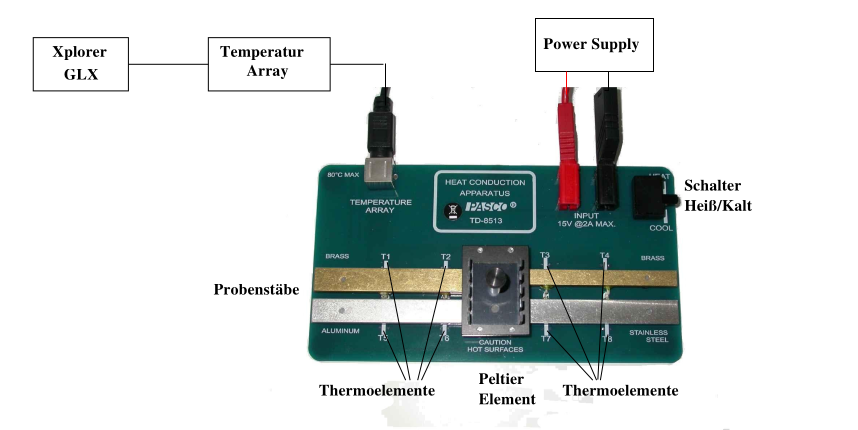
\includegraphics[scale=0.5]{content/pcb.png}
  \caption{Foto des Versuchsaufbaus.\cite{AP01}}
  \label{fig:aufbau}
\end{figure}

\subsection{Die statische Methode}
\label{sec:statisch}
Hier wird an zwei Punkten jeder Metallprobe die Temperatur als Funktion der Zeit
gemessen. Durch den aufgenommenen Temperaturverlauf wird die Wärmeleitfähigkeit bestimmt.
Der Datenlogger wird auf eine Abtastrate von $\Delta t_{GLX} = 10 \si{\second}$
gestellt. Die Sensoren werden im \textit{Home}-Verzeichnis unter dem Reiter \textit{Digital}
angezeigt. Das Netzteil wird auf eine Spannung von $U_P = 5 \si{\volt}$ eingestellt.
Die Messung wird beendet, wenn das Thermoelement $T7$ eine Temperatur von $45 \si{\celsius}$
anzeigt.

\subsection{Die dynamische Methode}
\label{sec:dynamisch}
Bei der dynamischen Methode oder dem Angström-Messverfahren wird der Probenstab
periodisch geheizt. Aus der Ausbreitungsgeschwindigkeit der Temperaturwelle lässt sich
dann die Wärmeleitfähigkeit bestimmen. Die Sensoren können wieder im Reiter \textit{Digital}
des Datenloggers eingesehen werden. Der Datenlogger wird auf eine Abtastrate von
$\Delta t_{GLX} = 2 \si{\second}$ eingestellt. Es wird eine Messung durchgeführt,
bei der die Probenelemente mit $80 \si{\second}$-Perioden geheizt und gekühlt werden.
Nun wird das Netzteil auf $U_P = 8 \si{\volt}$ und maximalen Strom eingestellt.
Die Messung wird erneut durchgeführt und erst bei mindestens $10$ Perioden eingestellt.
Eine dritte Messung wird mit einer Periodendauer von $200 \si{\second}$ durchgeführt.
Diese wird beendet, wenn eines der Probenelemente eine Temperatur von $80 \si{\celsius}$
erreicht. Anschließend werden die Elemente abgekühlt.
